\documentclass[11pt,compress,t,notes=noshow, xcolor=table]{beamer}
\usepackage[]{graphicx}\usepackage[]{color}
% maxwidth is the original width if it is less than linewidth
% otherwise use linewidth (to make sure the graphics do not exceed the margin)
\makeatletter
\def\maxwidth{ %
  \ifdim\Gin@nat@width>\linewidth
    \linewidth
  \else
    \Gin@nat@width
  \fi
}
\makeatother

\definecolor{fgcolor}{rgb}{0.345, 0.345, 0.345}
\newcommand{\hlnum}[1]{\textcolor[rgb]{0.686,0.059,0.569}{#1}}%
\newcommand{\hlstr}[1]{\textcolor[rgb]{0.192,0.494,0.8}{#1}}%
\newcommand{\hlcom}[1]{\textcolor[rgb]{0.678,0.584,0.686}{\textit{#1}}}%
\newcommand{\hlopt}[1]{\textcolor[rgb]{0,0,0}{#1}}%
\newcommand{\hlstd}[1]{\textcolor[rgb]{0.345,0.345,0.345}{#1}}%
\newcommand{\hlkwa}[1]{\textcolor[rgb]{0.161,0.373,0.58}{\textbf{#1}}}%
\newcommand{\hlkwb}[1]{\textcolor[rgb]{0.69,0.353,0.396}{#1}}%
\newcommand{\hlkwc}[1]{\textcolor[rgb]{0.333,0.667,0.333}{#1}}%
\newcommand{\hlkwd}[1]{\textcolor[rgb]{0.737,0.353,0.396}{\textbf{#1}}}%
\let\hlipl\hlkwb

\usepackage{framed}
\makeatletter
\newenvironment{kframe}{%
 \def\at@end@of@kframe{}%
 \ifinner\ifhmode%
  \def\at@end@of@kframe{\end{minipage}}%
  \begin{minipage}{\columnwidth}%
 \fi\fi%
 \def\FrameCommand##1{\hskip\@totalleftmargin \hskip-\fboxsep
 \colorbox{shadecolor}{##1}\hskip-\fboxsep
     % There is no \\@totalrightmargin, so:
     \hskip-\linewidth \hskip-\@totalleftmargin \hskip\columnwidth}%
 \MakeFramed {\advance\hsize-\width
   \@totalleftmargin\z@ \linewidth\hsize
   \@setminipage}}%
 {\par\unskip\endMakeFramed%
 \at@end@of@kframe}
\makeatother

\definecolor{shadecolor}{rgb}{.97, .97, .97}
\definecolor{messagecolor}{rgb}{0, 0, 0}
\definecolor{warningcolor}{rgb}{1, 0, 1}
\definecolor{errorcolor}{rgb}{1, 0, 0}
\newenvironment{knitrout}{}{} % an empty environment to be redefined in TeX

\usepackage{alltt}
\newcommand{\SweaveOpts}[1]{}  % do not interfere with LaTeX
\newcommand{\SweaveInput}[1]{} % because they are not real TeX commands
\newcommand{\Sexpr}[1]{}       % will only be parsed by R
\newcommand{\xmark}{\ding{55}}%


\usepackage[english]{babel}
\usepackage[utf8]{inputenc}

\usepackage{dsfont}
\usepackage{verbatim}
\usepackage{amsmath}
\usepackage{amsfonts}
\usepackage{amssymb}
\usepackage{bm}
\usepackage{csquotes}
\usepackage{multirow}
\usepackage{longtable}
\usepackage{booktabs}
\usepackage{enumerate}
\usepackage[absolute,overlay]{textpos}
\usepackage{psfrag}
\usepackage{algorithm}
\usepackage{algpseudocode}
\usepackage{eqnarray}
\usepackage{arydshln}
\usepackage{tabularx}
\usepackage{placeins}
\usepackage{tikz}
\usepackage{setspace}
\usepackage{colortbl}
\usepackage{mathtools}
\usepackage{wrapfig}
\usepackage{bm}
\usepackage{amsmath}
\usepackage{pifont}
\usepackage{xcolor} %colored math symbols

\usetikzlibrary{shapes,arrows,automata,positioning,calc,chains,trees, shadows}
\tikzset{
  %Define standard arrow tip
  >=stealth',
  %Define style for boxes
  punkt/.style={
    rectangle,
    rounded corners,
    draw=black, very thick,
    text width=6.5em,
    minimum height=2em,
    text centered},
  % Define arrow style
  pil/.style={
    ->,
    thick,
    shorten <=2pt,
    shorten >=2pt,}
}

\usepackage{subfig}

% Defines macros and environments
\usepackage{../../style/lmu-lecture}


\let\code=\texttt
\let\proglang=\textsf

\setkeys{Gin}{width=0.9\textwidth}

\setbeamertemplate{frametitle}{\expandafter\uppercase\expandafter\insertframetitle}

\usepackage{bbm}
% basic latex stuff
\newcommand{\pkg}[1]{{\fontseries{b}\selectfont #1}} %fontstyle for R packages
\newcommand{\lz}{\vspace{0.5cm}} %vertical space
\newcommand{\dlz}{\vspace{1cm}} %double vertical space
\newcommand{\oneliner}[1] % Oneliner for important statements
{\begin{block}{}\begin{center}\begin{Large}#1\end{Large}\end{center}\end{block}}


%new environments
\newenvironment{vbframe}  %frame with breaks and verbatim
{
 \begin{frame}[containsverbatim,allowframebreaks]
}
{
\end{frame}
}

\newenvironment{vframe}  %frame with verbatim without breaks (to avoid numbering one slided frames)
{
 \begin{frame}[containsverbatim]
}
{
\end{frame}
}

\newenvironment{blocki}[1]   % itemize block
{
 \begin{block}{#1}\begin{itemize}
}
{
\end{itemize}\end{block}
}

\newenvironment{fragileframe}[2]{  %fragile frame with framebreaks
\begin{frame}[allowframebreaks, fragile, environment = fragileframe]
\frametitle{#1}
#2}
{\end{frame}}


\newcommand{\myframe}[2]{  %short for frame with framebreaks
\begin{frame}[allowframebreaks]
\frametitle{#1}
#2
\end{frame}}

\newcommand{\remark}[1]{
  \textbf{Remark:} #1
}


\newenvironment{deleteframe}
{
\begingroup
\usebackgroundtemplate{
\includegraphics[width=\paperwidth,height=\paperheight]{../style/color/red.png}}
 \begin{frame}
}
{
\end{frame}
\endgroup
}
\newenvironment{simplifyframe}
{
\begingroup
\usebackgroundtemplate{
\includegraphics[width=\paperwidth,height=\paperheight]{../style/color/yellow.png}}
 \begin{frame}
}
{
\end{frame}
\endgroup
}\newenvironment{draftframe}
{
\begingroup
\usebackgroundtemplate{
\includegraphics[width=\paperwidth,height=\paperheight]{../style/color/green.jpg}}
 \begin{frame}
}
{
\end{frame}
\endgroup
}
% https://tex.stackexchange.com/a/261480: textcolor that works in mathmode
\makeatletter
\renewcommand*{\@textcolor}[3]{%
  \protect\leavevmode
  \begingroup
    \color#1{#2}#3%
  \endgroup
}
\makeatother


\input{../../latex-math/basic-math}
\input{../../latex-math/basic-ml}
\input{../../latex-math/ml-nn}

\newcommand{\titlefigure}{figure/rosenblatt_perceptron.jpg}
\newcommand{\learninggoals}{
  \item Predecessors of modern (deep) neural networks
  \item History of DL as a field
}

\title{Deep Learning}
\date{}

\begin{document}

\lecturechapter{Brief History}
\lecture{I2DL}
%%%%%%%%%%%%%%%%%%%%%%%%%%%%%%%%%%%%%%%%%%%%%%%%%%%%%%%%%%%%%%%%%%

\begin{vbframe}{A brief history of neural networks}
\begin{itemize}
\item \pkg{1943:} The first artificial neuron, the "Threshold Logic Unit (TLU)", was proposed by Warren McCulloch \& Walter Pitts.
\begin{figure}
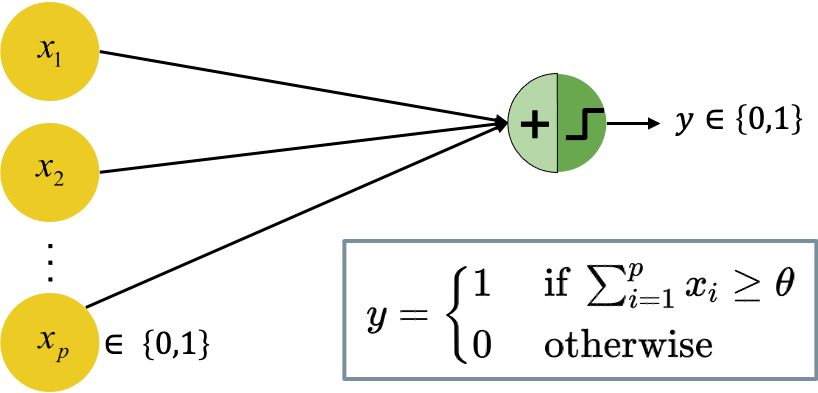
\includegraphics[width=7cm]{figure/mp_neuron.png}
\end{figure}
\begin{itemize}
\item The model is limited to binary inputs.
\vspace{2mm}
\item %The MP-neuron 
It fires/outputs  $+1$ if the input exceeds a certain threshold $\theta$.
\vspace{2mm}
\item The weight are not adjustable, so learning could only be achieved by changing the threshold $\theta$.
\end{itemize}
\end{itemize}
\framebreak
%%%%%%%%%%%%%%%%%%%%%%%%%%%%%%%%%%%%%%%%%%%%%%%%%%%%%%%%%%%%%%%%%%  

\begin{itemize}
\item \pkg{1957:} The perceptron was invented by Frank Rosenblatt. 
\begin{figure}
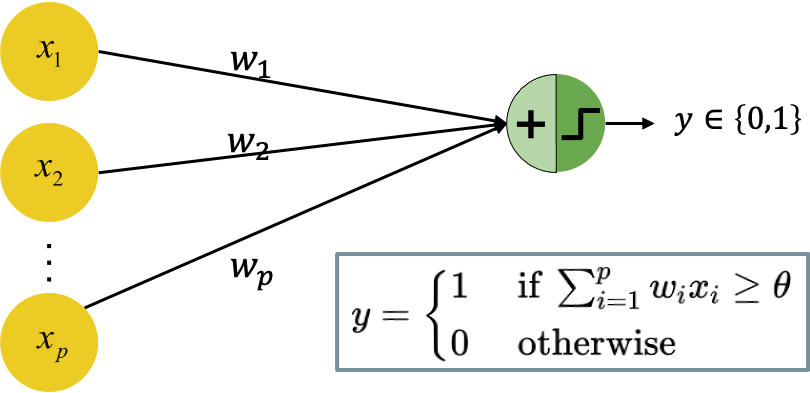
\includegraphics[width=7cm]{figure/perceptron_new.png}
\end{figure}
\begin{itemize}
\vspace{2mm}
\item The inputs are not restricted to be binary.
\vspace{2mm}
\item %In perceptron, 
The weights are adjustable and can be learned by learning algorithms.
\vspace{2mm}
\item %5Similar to the% MP-neuron
As for the TLU, the threshold is adjustable and decision boundaries are linear.
\end{itemize}
\end{itemize}
\framebreak
%%%%%%%%%%%%%%%%%%%%%%%%%%%%%%%%%%%%%%%%%%%%%%%%%%%%%%%%%%%%%%%%%%

\begin{itemize}
\item \pkg{1960:} Adaptive Linear Neuron (ADALINE) was invented by Bernard Widrow \& Ted Hoff; weights are now adjustable according to the weighted sum of the inputs.
\vspace{.1cm}
\begin{figure}
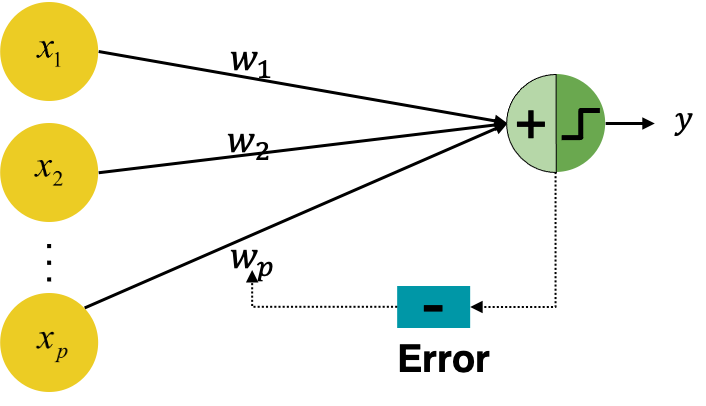
\includegraphics[width=6cm]{figure/adaline.png}
\end{figure}
%\vspace{1cm}
\item \pkg{1965:} Group method of data handling (also known as polynomial neural networks) by Alexey Ivakhnenko. The first learning algorithm for supervised deep feedforward multilayer perceptrons.
\framebreak
%%%%%%%%%%%%%%%%%%%%%%%%%%%%%%%%%%%%%%%%%%%%%%%%%%%%%%%%%%%%%%%%%%

\item \pkg{1969:} The first \enquote{AI Winter} kicked in.
\begin{itemize}
\item Marvin Minsky \& Seymour Papert proved that a perceptron cannot solve the XOR-Problem (linear separability).
\item Less funding $\Rightarrow$ Standstill in AI/DL research.
\end{itemize}
\end{itemize}
\begin{figure}
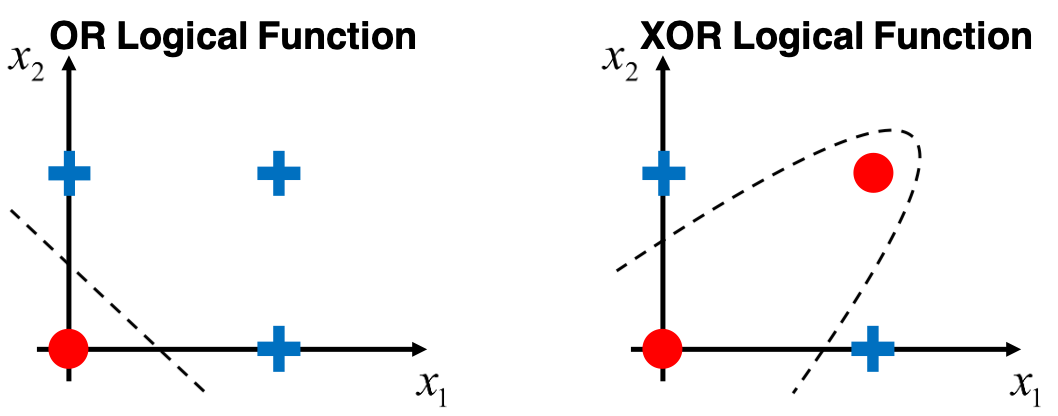
\includegraphics[width=7cm]{figure/orvsxor.png}
\end{figure}
\begin{itemize}
\item \pkg{1985:} Multilayer perceptron with backpropagation by David Rumelhart, Geoffrey Hinton, and Ronald Williams.
\begin{itemize}
\item Efficiently compute derivatives of composite functions.
\item Backpropagation was developed already in 1970 by Linnainmaa.
\end{itemize}
\framebreak
%%%%%%%%%%%%%%%%%%%%%%%%%%%%%%%%%%%%%%%%%%%%%%%%%%%%%%%%%%%%%%%%%%

\item \pkg{1985:} The second \enquote{AI Winter} kicked in.

\begin{itemize}
\footnotesize\item Overly optimistic expectations concerning potential of AI/DL.
\footnotesize\item The phrase \enquote{AI} even reached a pseudoscience status.
\footnotesize\item Kernel machines and graphical models both achieved good results on many important tasks.
\footnotesize\item Some fundamental mathematical difficulties in modeling long sequences were identified.
\end{itemize}
\begin{figure}
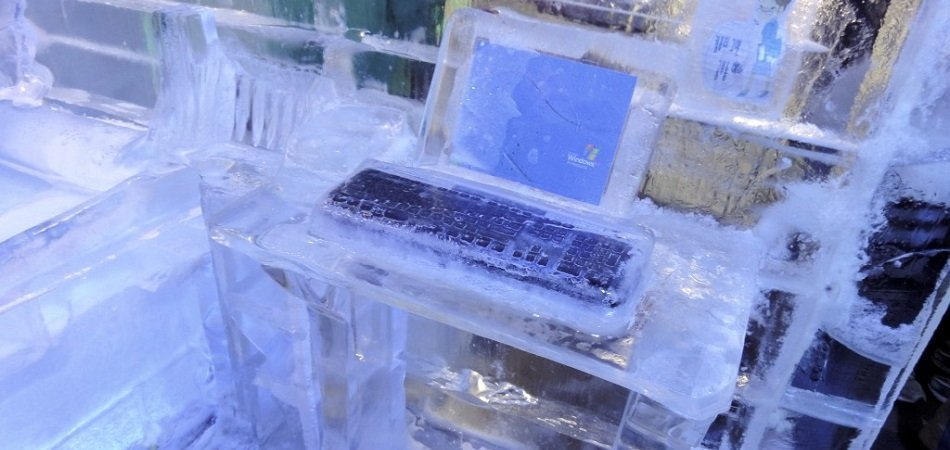
\includegraphics[width=8cm]{figure/ai_winter.jpg}
\\
\tiny{Credit: https://emerj.com/ai-executive-guides/will-there-be-another-artificial-intelligence-winter-probably-not/}
\end{figure}
\framebreak
%%%%%%%%%%%%%%%%%%%%%%%%%%%%%%%%%%%%%%%%%%%%%%%%%%%%%%%%%%%%%%%%%%

\item \pkg{2006:} Age of deep neural networks began.

\begin{itemize}
\footnotesize\item Geoffrey Hinton showed that a deep belief network could be efficiently trained using \textit{greedy layer-wise pretraining}.
\footnotesize\item This wave of research popularized the use of the term deep learning to emphasize that researchers were now able to train deeper neural networks than had been possible before.
\footnotesize\item At this time, deep neural networks outperformed competing AI systems based on other ML technologies as well as hand-designed functionality.
\end{itemize}
\begin{figure}
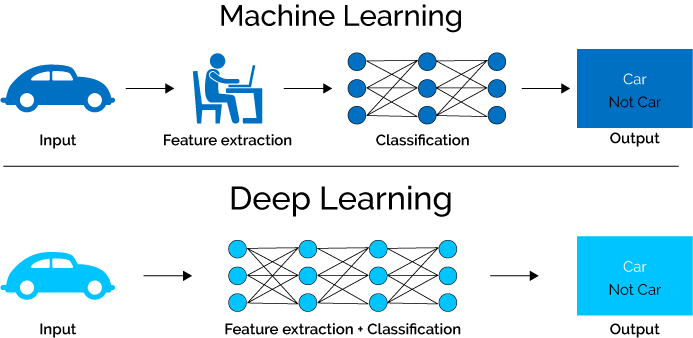
\includegraphics[width=9cm]{figure/dl_feature2.png}

\end{figure}
\end{itemize}
\framebreak
%%%%%%%%%%%%%%%%%%%%%%%%%%%%%%%%%%%%%%%%%%%%%%%%%%%%%%%%%%%%%%%%%%

%\textbf{Why now and not earlier?}
%\begin{enumerate}
%\vspace{2mm}
%\item Significantly bigger datasets.
%\vspace{2mm}
%\item Better algorithms resolving the vanishing gradient problem.
%\vspace{2mm}
%\item Better regularization.
%\vspace{2mm}
%\item Unsupervised representation learning.
%\vspace{2mm}
%\item More layers lead to a significant increase of parameters.
%\vspace{2mm}
%\item Deep neural networks are trained on GPUs, rather than CPUs. So processing power can handle huge amounts of parameters.
%\vspace{2mm}
%\item Investment by industries and universities.
%\vspace{2mm}
%\item DL tools make learning and applying DL easier.
%\end{enumerate}
%\framebreak
%%%%%%%%%%%%%%%%%%%%%%%%%%%%%%%%%%%%%%%%%%%%%%%%%%%%%%%%%%%%%%%%%%

\begin{figure}
\centering
\scalebox{1.1}{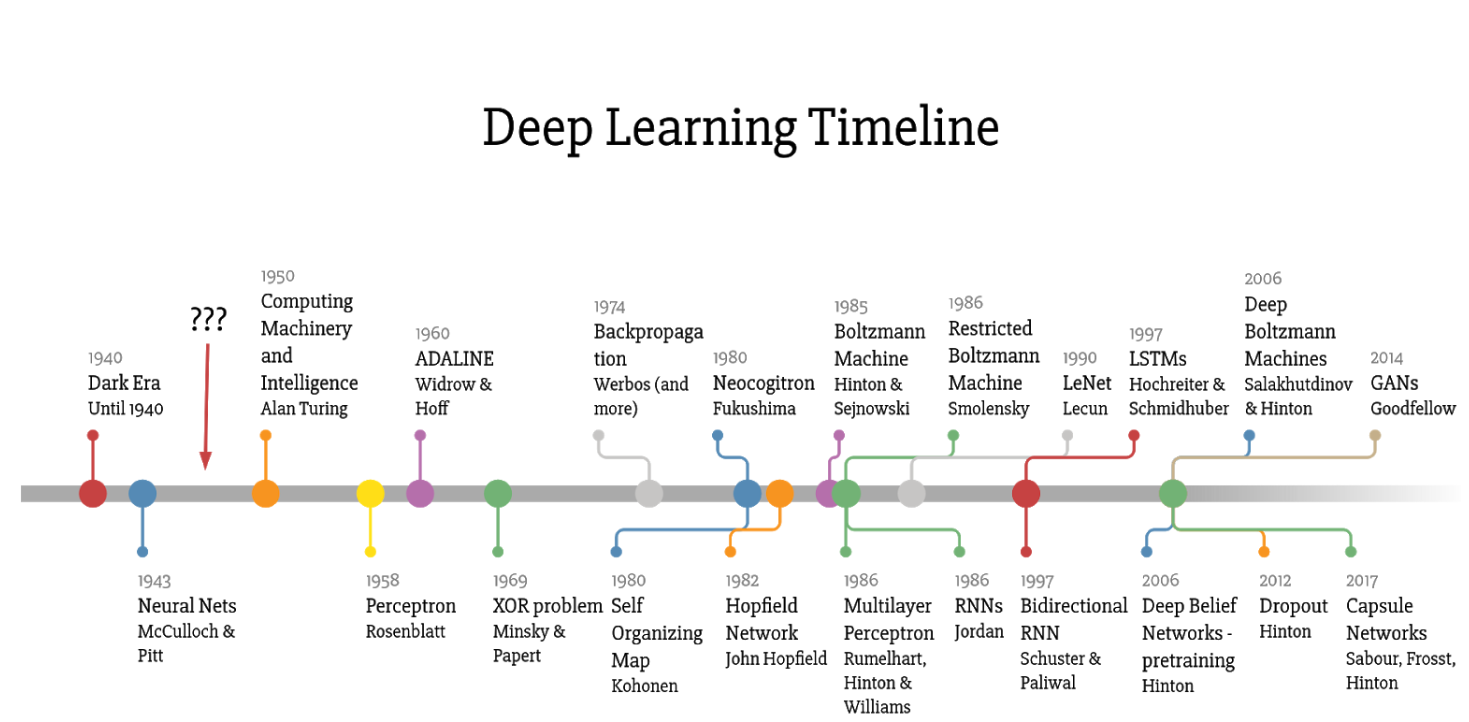
\includegraphics{figure/dl_timeline.png}}
\vspace{.5cm}
\tiny{Credit: https://towardsdatascience.com/a-weird-introduction-to-deep-learning-7828803693b0}
\framebreak
%%%%%%%%%%%%%%%%%%%%%%%%%%%%%%%%%%%%%%%%%%%%%%%%%%%%%%%%%%%%%%%%%%

\scalebox{1.1}{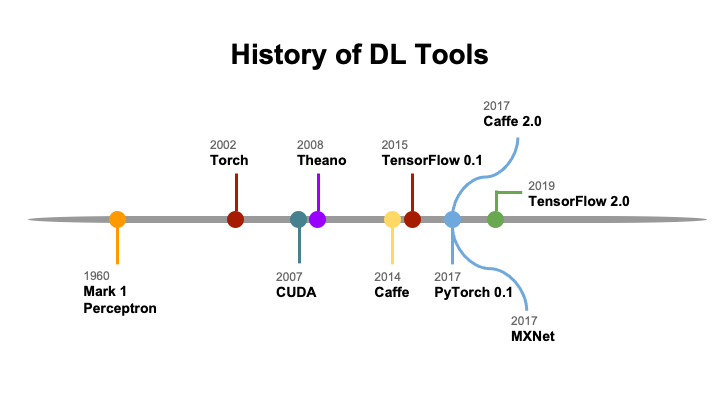
\includegraphics{figure/DL_tools.png}}
\end{figure}
\framebreak
%%%%%%%%%%%%%%%%%%%%%%%%%%%%%%%%%%%%%%%%%%%%%%%%%%%%%%%%%%%%%%%%%%

%\begin{figure}
%\centering
%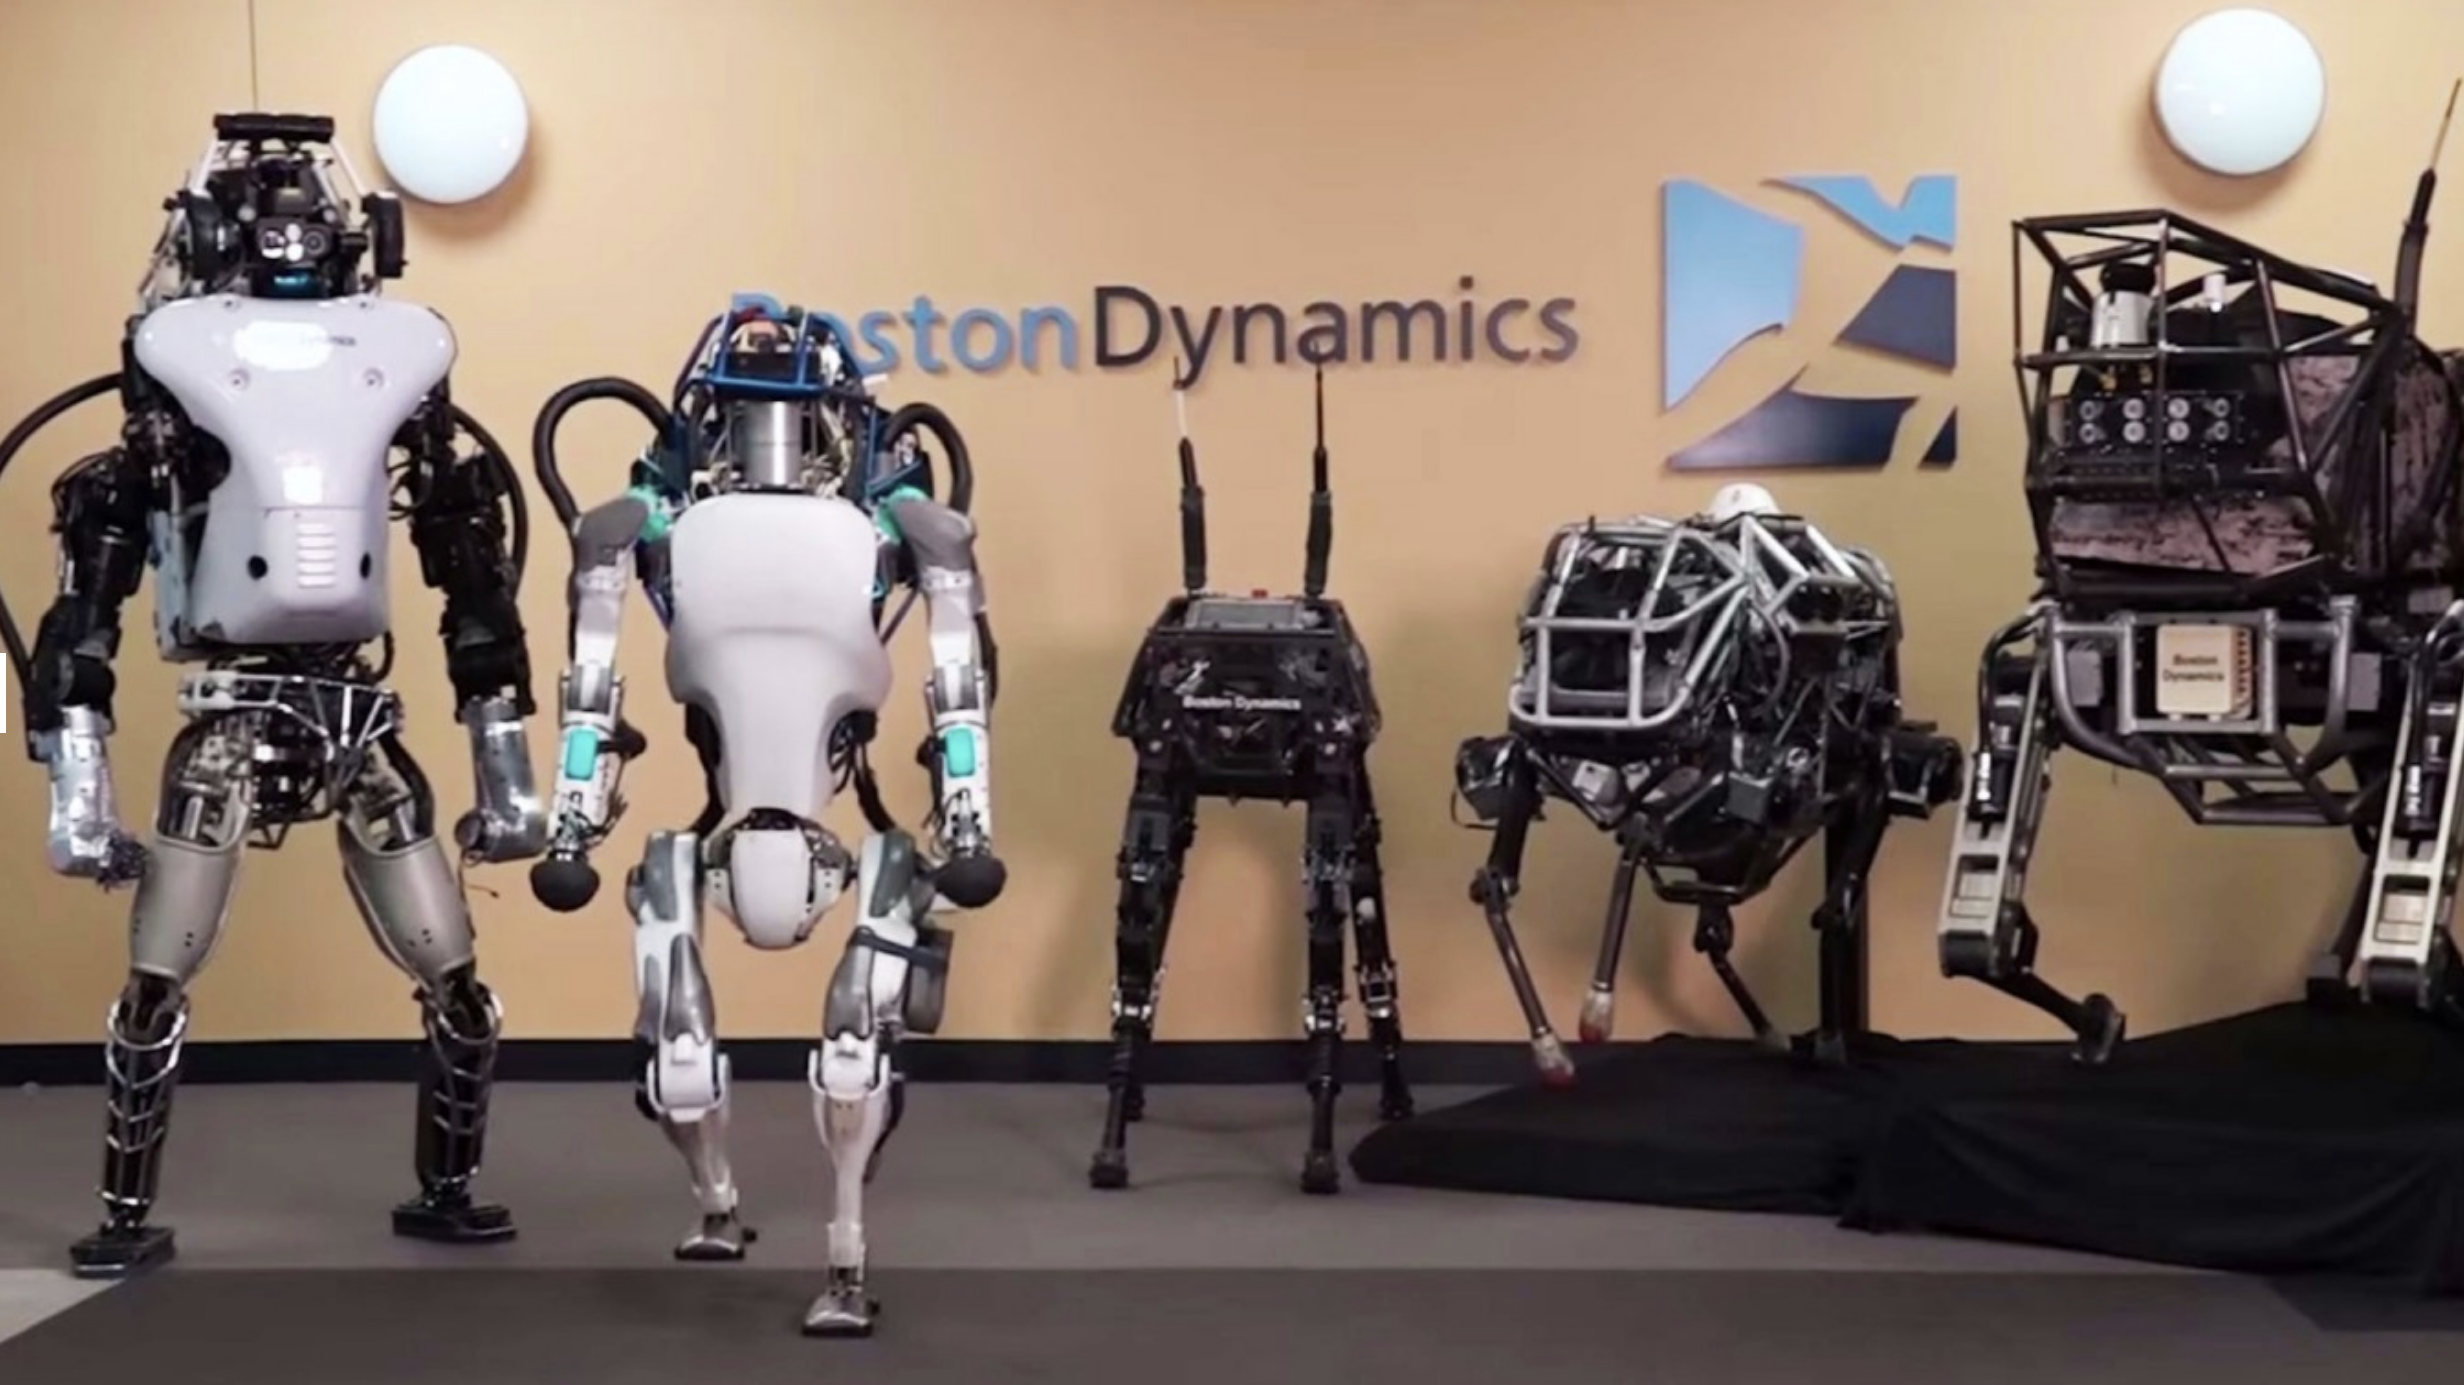
\includegraphics[width=8cm]{figure/bostondynamic.png}
%\caption{Boston Dynamics (\href{https://www.youtube.com/watch?v=fUyU3lKzoio&ab_channel=BostonDynamics}{click here})}
%\end{figure}
%\footnotesize
%\begin{itemize}
%\item Boston Dynamics is a world leader in mobile robots founded in 1992 as a spin-off from the Massachusetts Institute of Technology.
%\vspace{.1cm}
%\item The company is best known for the development of a series of dynamic highly-mobile robots, including BigDog, Spot, Atlas, and Handle.
%\end{itemize}
%\framebreak
%%%%%%%%%%%%%%%%%%%%%%%%%%%%%%%%%%%%%%%%%%%%%%%%%%%%%%%%%%%%%%%%%%

\begin{figure}
\centering
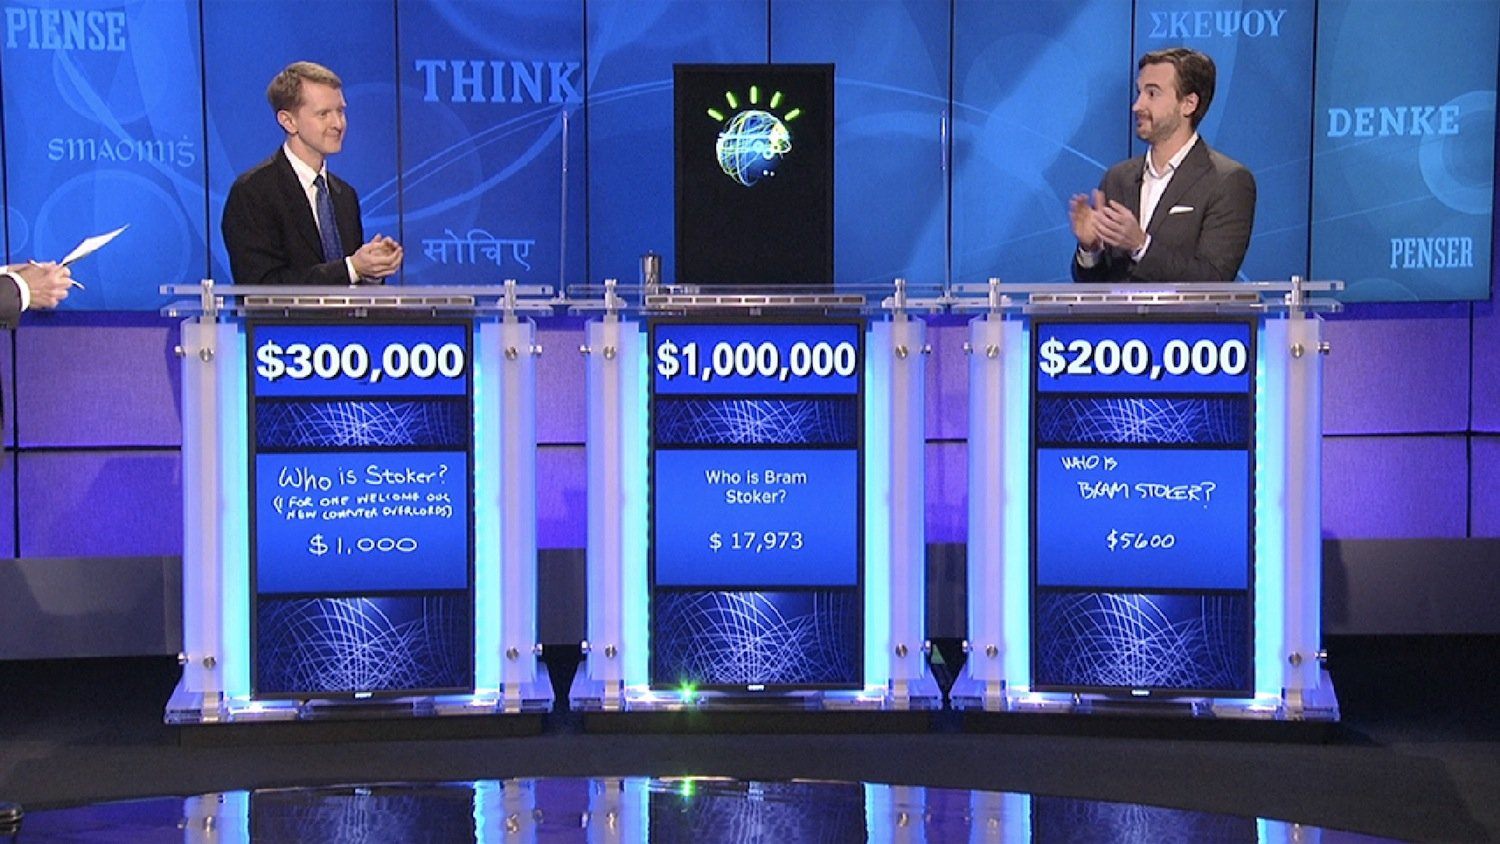
\includegraphics[width=8cm]{figure/ibmsupercomputer.jpg}
\caption{IBM Supercomputer}
\end{figure}
\footnotesize
\begin{itemize}
\item Watson is a question-answering system capable of answering questions posed in natural language, developed in IBM's DeepQA project.
\vspace{.1cm}
\item In 2011, Watson competed on \textit{Jeopardy!} against champions Brad Rutter and Ken Jennings, winning the first place prize of $\$ 1$ million.
\end{itemize}
\framebreak
%%%%%%%%%%%%%%%%%%%%%%%%%%%%%%%%%%%%%%%%%%%%%%%%%%%%%%%%%%%%%%%%%%

\begin{figure}
\centering
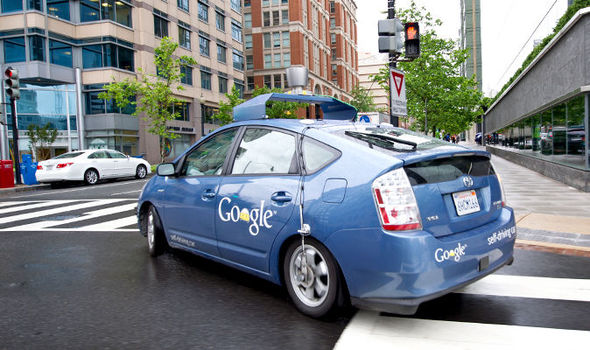
\includegraphics[width=7cm]{figure/selfdriving.jpg}
\caption{Google self driving car (Waymo)}
\end{figure}
\footnotesize
\begin{itemize}
\item Google's development of self-driving technology began on January 17, 2009, at the company's secretive X lab.
\vspace{.1cm}
\item By January 2020, $20$ million miles of self-driving on public roads had been completed by Waymo.
\end{itemize}
\framebreak
%%%%%%%%%%%%%%%%%%%%%%%%%%%%%%%%%%%%%%%%%%%%%%%%%%%%%%%%%%%%%%%%%%

\begin{figure}
\centering
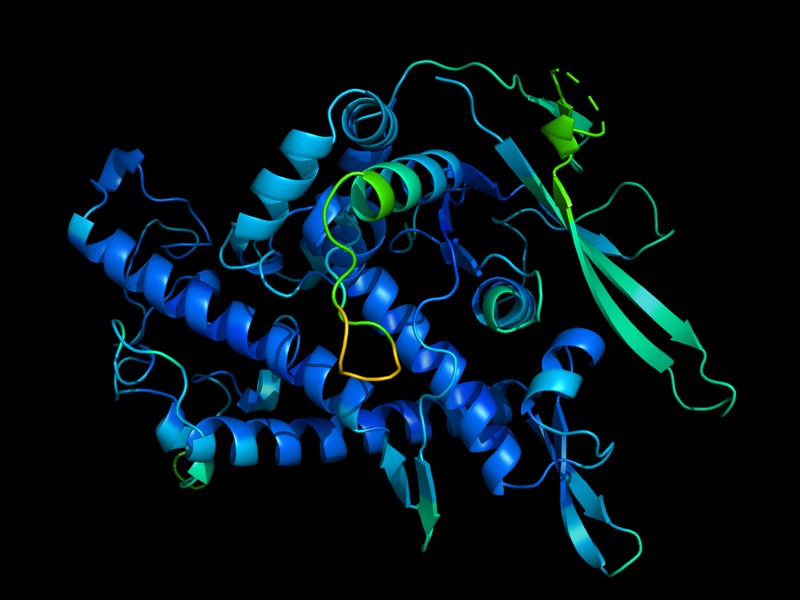
\includegraphics[width=7cm]{figure/alphafold.jpg}
\\
\tiny {Credit: DeepMind}
\end{figure}
\footnotesize
\begin{itemize}
\item\textbf{AlphaFold} is a deep learning system, developed by Google DeepMind, for determining a protein's 3D shape from its amino-acid sequence.
\vspace{.1cm}
\item In 2018 and 2020, AlphaFold placed first in the overall rankings of the Critical Assessment of Techniques for Protein Structure Prediction (CASP).
\end{itemize}
\framebreak
%%%%%%%%%%%%%%%%%%%%%%%%%%%%%%%%%%%%%%%%%%%%%%%%%%%%%%%%%%%%%%%%%%
\begin{figure}
\centering
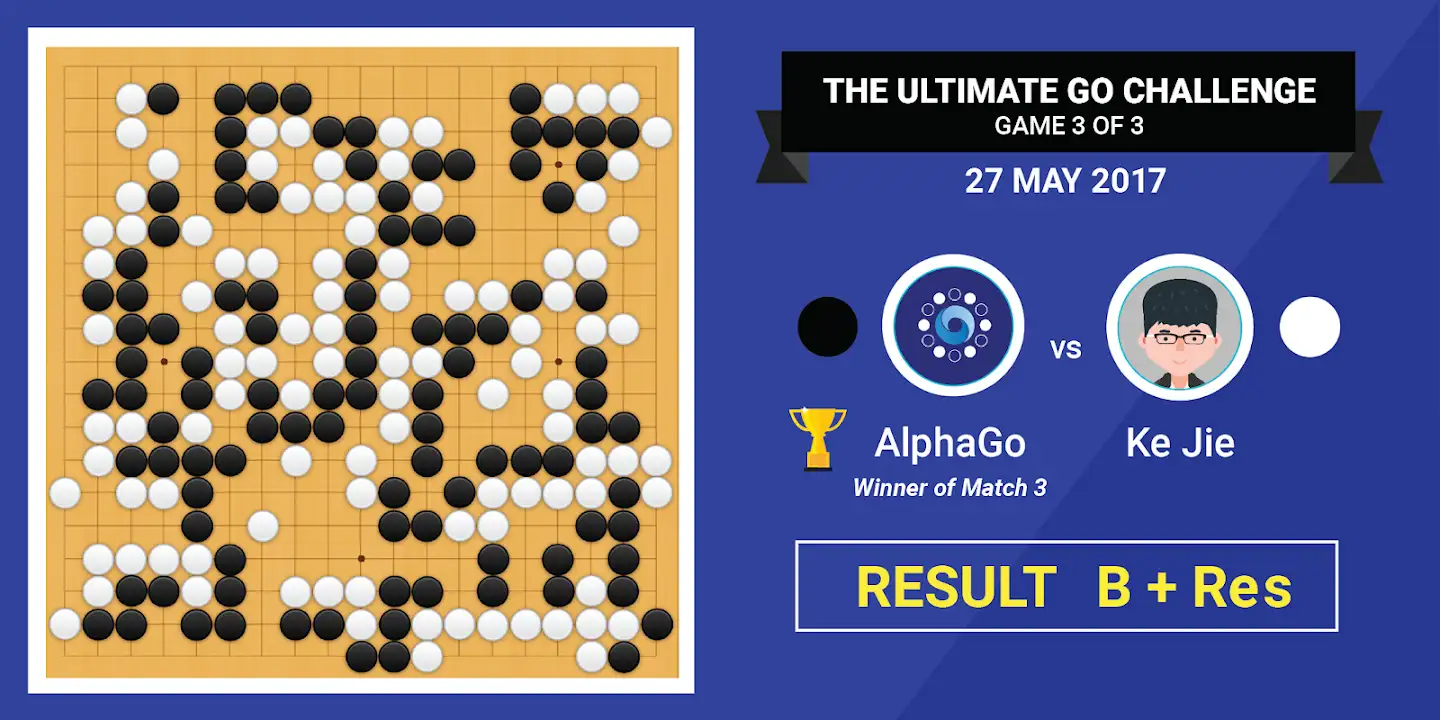
\includegraphics[width=8cm]{figure/alphago.png}
\\
\tiny {Credit: DeepMind}
\end{figure}
\footnotesize
\begin{itemize}
\item\textbf{AlphaGo}, originally developed by DeepMind, is a deep learning system that plays the board game Go. In 2017, the Master version of AlphaGo beat Ke Jie, the number one ranked player in the world at the time.
\vspace{.1cm}
\item While there are several extensions to AlphaGo (e.g., Master AlphaGo, AlphaGo Zero, AlphaZero, and MuZero), the main idea is the same: search for optimal moves based on knowledge acquired by machine learning.
\end{itemize}
\framebreak
%%%%%%%%%%%%%%%%%%%%%%%%%%%%%%%%%%%%%%%%%%%%%%%%%%%%%%%%%%%%%%%%%%

\begin{figure}
\centering
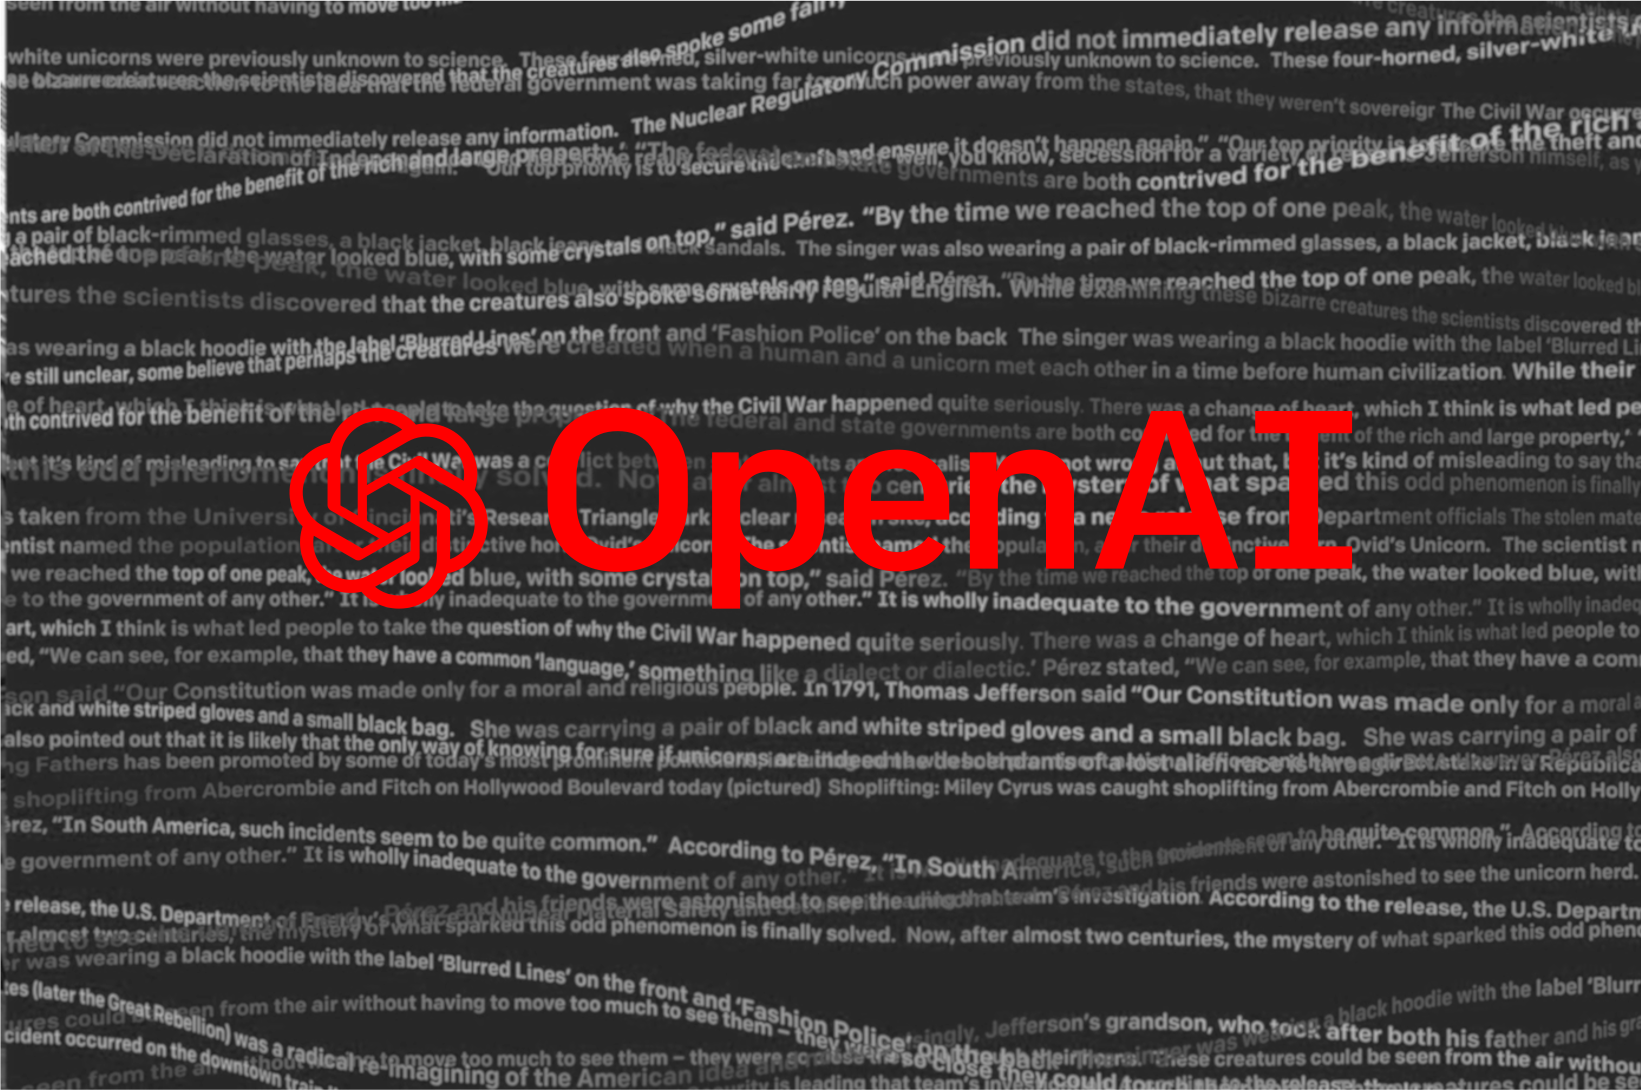
\includegraphics[width=7cm]{figure/gpt3.png}
\end{figure}
\footnotesize
\begin{itemize}
\item\textbf{Generative Pre-trained Transformer 3 (GPT-3)} is the third generatation of the GPT model, introduced by OpenAI in May 2020, to produce human-like text.
\vspace{.1cm}
\item There are 175 billion parameters to be learned by the algorithm, but the quality of the generated text is so high that it is hardly possible to distinguish it from a human-written text.
\end{itemize}
\end{vbframe}
%%%%%%%%%%%%%%%%%%%%%%%%%%%%%%%%%%%%%%%%%%%%%%%%%%%%%%%%%%%%%%%%%%

\endlecture
\end{document}